\section{Lenguajes y entornos}

En el desarrollo se han usado una serie de lenguajes y entornos con los que se ha desarrollado el proyecto entero, entendiéndose por esto la aplicación móvil, la \acrshort{api} y este documento.

\subsection{LaTeX}
\label{lib:latex}

\begin{wrapfigure}[6]{r}{0.2\textwidth}
    \vspace{-20pt}
    \centering
    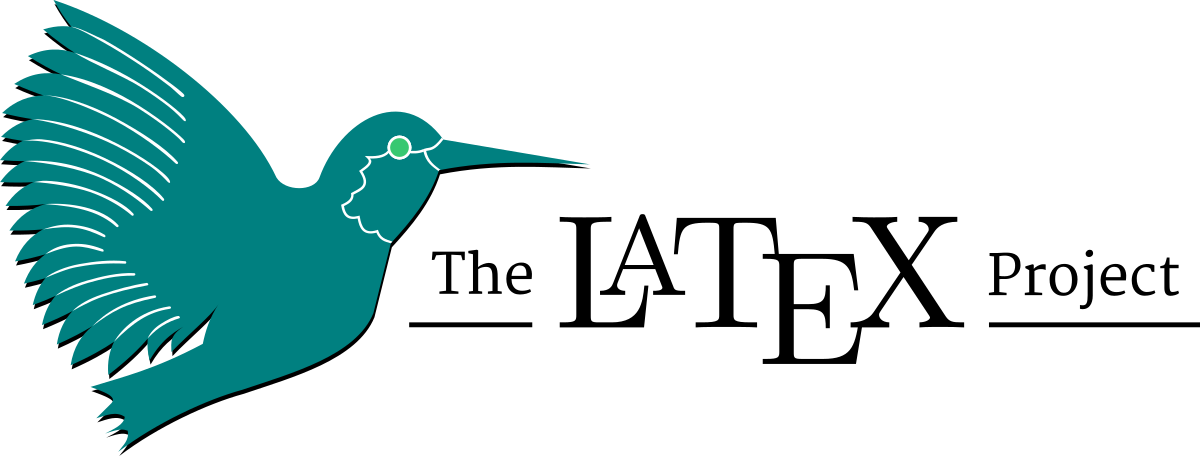
\includegraphics[width=0.2\textwidth]{Implementación/latex-icon.png}
    \vspace{-20pt}
    \caption{Logo de LaTeX}
\end{wrapfigure}

LaTeX es un sistema para la \textbf{elaboración de documentos} por medio de texto plano a diferencia del texto formateado que se produce en otros softwares de creación de documentos. Es un software gratuito y el estándar de facto para la comunicación y publicación de documentos científicos a día de hoy. LaTeX ha sido empleado en la \textbf{redacción de este documento}.

Para más información: \href{https://www.latex-project.org/}{https://www.latex-project.org/}

\subsection{Kotlin}
\label{lib:kotlin}

\begin{wrapfigure}[6]{l}{0.2\textwidth}
    \vspace{-15pt}
    \centering
    
\includegraphics[width=0.15\textwidth]{Implementación/kotlin-icon.jpg}
    \vspace{-10pt}
    \caption{Logo de Kotlin}
\end{wrapfigure}

Kotlin es un lenguaje de programación desarrollado por \textbf{JetBrains} con aportaciones comunitarias. Es un lenguaje de tipado estático para programación de propósito general multiplataforma. 

Entre sus principales características se encuentran la interorperabilidad total con Java y la \acrshort{jvm} (y por tanto con Spring o Micronaut), la inferencia de tipos, su capacidad de compilación a código Javascript o que, desde el año 2019, Kotlin es el lenguaje de desarrollo elegido por Google como \textbf{primera opción para Android}\cite{kotlin2019}. Siguiendo esto, Kotlin ha sido empleado en este proyecto en el \textbf{desarrollo de la aplicación móvil}.

Para más información: \href{https://kotlinlang.org/}{https://kotlinlang.org/}

\subsection{Node}
\label{lib:node}

Desarrollado y lanzado por \textbf{Ryan Dahl} en 2009, Node.js es un entorno multiplataforma de back-end de Javascript. Es de código abierto y a día es mantenido por la \textbf{OpenJS Foundation}, la misma fundación que mantiene jQuery o webpack entre otros proyectos.

\begin{wrapfigure}[6]{r}{0.2\textwidth}
    \vspace{-5pt}
    \centering
    
\includegraphics[width=0.18\textwidth]{Implementación/node-icon.png}
    \vspace{-10pt}
    \caption{Logo de Node.js}
\end{wrapfigure}

Este entorno permite a los desarrolladores crear aplicaciones en el lado del servidor con un lenguaje inicialmente concebido para ser client-side. De esta forma Node.js permite el \textbf{desarrollo de aplicaciones web íntegramente en Javascript}. Tiene una arquitectura basada en eventos con entradas y salidas asíncronas. A día de hoy se encuentra en la versión 17, teniendo Node.js 16 como su versión de largo soporte activa actualmente.

Para más información: \href{https://nodejs.org/en/}{https://nodejs.org/en/}

\subsection{TypeScript}
\label{lib:typescript}

TypeScript es un superset de Javascript desarrollado y mantenido por \textbf{Microsoft}. Su sintaxis contiene todo lo que contiene Javascript con el añadido de tipado estático opcional. El código de TypeScript se \textbf{compila a código Javascript}, que es el código finalmente ejecutado. Su premisa nace de dotar de mayor seguridad y validación a los desarrollos con Javascript.

\begin{wrapfigure}[6]{l}{0.2\textwidth}
    \vspace{-25pt}
    \centering
    
\includegraphics[width=0.15\textwidth]{Implementación/ts-icon.png}
    \vspace{-10pt}
    \caption{Logo de TypeScript}
\end{wrapfigure}

Al cimentarse sobre Javascript, TypeScript es también un lenguaje multiparadigama que permite la programación funcional, imperativa y orientada a objetos. Es compatible con todas las librerías de Javascript aunque no estén escritas en TypeScript, permitiendo incluso dotarlas de las capacidades de este lenguaje por medio del uso de \textbf{archivos de definición de tipos} que añade esos tipos sobre código Javascript, sea ajeno o propio. En los últimos años, TypeScript ha sido el lenguaje con mayor crecimiento en uso como demuestra su presencia en GitHub\cite{octoverse2021}.

Para más información: \href{https://www.typescriptlang.org/}{https://www.typescriptlang.org/}